\documentclass[11pt,a4paper]{article}

% --- PACOTES ---
\usepackage[utf8]{inputenc}
\usepackage[brazil]{babel}
\usepackage[margin=1in]{geometry}
\usepackage{amsmath,amssymb}
\usepackage{graphicx}
\usepackage{booktabs}
\usepackage{xcolor}
\usepackage{hyperref}
\usepackage{microtype}
\usepackage{caption}
\usepackage{subcaption}
\usepackage{enumitem}
\usepackage{titlesec}

% Cores Oficiais
\definecolor{apartblue}{RGB}{0, 114, 178}
\definecolor{darkblue}{RGB}{15, 34, 64}
\definecolor{boxbg}{RGB}{244, 246, 249}

\hypersetup{
    colorlinks=true,
    linkcolor=apartblue,
    citecolor=apartblue,
    urlcolor=apartblue
}

\titleformat{\section}{\large\bfseries\color{darkblue}}{\thesection.}{0.5em}{}
\titleformat{\subsection}{\normalsize\bfseries\color{apartblue}}{\thesubsection}{0.5em}{}

% --- TÍTULO E AUTORES ---
\title{\vspace{-1.5cm}\textbf{\Large Tempo até o Colapso e Governança Emergente: \\ Como Desertores Gananciosos Desestabilizam a Evolução de Normas em Bens Comuns de LLMs}}
\author{
    \textbf{[Nome do Autor 1]} \thanks{[Filiação / Instituição 1]} \and
    \textbf{[Nome do Autor 2]} \thanks{[Filiação / Instituição 2]}
}
\date{\textit{Swarm Alignment Hackathon --- Apart Research (Novembro de 2026)}}

\begin{document}

\maketitle

\vspace{-0.5cm}
\begin{center}
\fcolorbox{apartblue}{boxbg}{
\begin{minipage}{0.94\textwidth}
\vspace{0.2cm}
\textbf{\color{apartblue}Resumo} \vspace{0.1cm} \\
\small
À medida que sistemas descentralizados multiagente baseados em LLMs são progressivamente implementados em ambientes de recursos compartilhados e finitos, a capacidade de estabelecer e sustentar governança coletiva torna-se imperativa para o alinhamento de enxames (\textit{swarm alignment}). Avaliando a gestão de bens comuns sob tomada de decisão simultânea, investigamos como enxames cooperativos de LLMs governam recursos compartilhados e respondem à intrusão abrupta de um agente recém-chegado (\textit{newcomer}) não alinhado e predatório. Replicando o arcabouço pesqueiro GovSim com um modelo de pesos abertos (\texttt{qwen2.5:7b}, 40 simulações concluídas ao longo de 15 sementes), demonstramos que a comunicação aliada a prompts de universalização sustenta os bens comuns ao longo de horizontes de 12 meses. A introdução de um agente ganancioso no Mês 4 reduz bruscamente a sobrevivência coletiva: a sobrevivência no marco temporal cai de 88\% nos controles para 33\% (teste exato de Fisher $p = 0,028$). Crucialmente, a degradação ocorre sem contágio comportamental: os agentes incumbentes não copiam a extração predatória, reduzindo as toneladas solicitadas. Expandindo além da exaustão física, revelamos um mecanismo institucional inédito: enxames cooperativos exibem espontaneamente aperto normativo adaptativo (Princípio 2 de Elinor Ostrom), reduzindo progressivamente os limites por agente de 10 para 1--4 t/mês para construir uma margem de segurança ecológica. O desertor quebra essa convergência, forçando os enxames sobreviventes à inflação de normas (slopes revertendo de $-0,24$ para $+0,68$ t/mês, $p = 0,006$). Esses resultados provam que o alinhamento em enxames não falha por trapaça interna, mas pela destruição do capital institucional acumulado.
\vspace{0.2cm}
\end{minipage}
}
\end{center}
\vspace{0.3cm}

\section{Introdução}
Uma questão fundamental no alinhamento de enxames (\textit{swarm alignment}) consiste em determinar se agentes autônomos de IA, operando em redes abertas e descentralizadas, conseguem estabelecer normas sociais duradouras para prevenir o esgotamento catastrófico de recursos compartilhados (a Tragédia dos Comuns). Enquanto o alinhamento de agentes individuais enfatiza a obediência a instruções e a inofensividade, o alinhamento multiagente introduz fenômenos em nível macro: coordenação na teoria dos jogos, credibilidade na comunicação, pressão social entre pares e resiliência institucional contra agentes oportunistas não alinhados (Dafoe et al., 2020; Park et al., 2023).

Um modelo central de ameaça em enxames autônomos reside na dinâmica da ``maçã podre'' (\textit{bad apple}): um grupo de agentes cooperativos e comunicativos consegue resistir à infiltração súbita de um desertor focado na maximização de retorno imediato? Caso os agentes incumbentes copiem prontamente o comportamento predatório (contágio comportamental), a coesão social colapsa de imediato. Por outro lado, caso os incumbentes mantenham a adesão aos acordos coletivos, a questão estrutural passa a ser se os mecanismos descentralizados de governança possuem capacidade adaptativa suficiente para absorver choques exógenos de deserção.

Neste trabalho, realizamos uma avaliação empírica aprofundada utilizando o ambiente GovSim (Piatti et al., 2024), avaliando um modelo de pesos abertos de 7 bilhões de parâmetros (Qwen 2.5 7B) em 40 simulações de longo horizonte. Nossas contribuições principais são:
\begin{enumerate}[leftmargin=*,itemsep=1pt]
    \item \textbf{Replicação em Pesos Abertos e Robustez de Benchmark:} Demonstramos que prompts de universalização combinados com diálogo mensal em linguagem natural sustentam recursos comuns em modelos locais abertos (\texttt{qwen2.5:7b}), atingindo 54\% de sobrevivência em 12 meses contra 0\% no baseline sem comunicação ($p = 5,4 \times 10^{-6}$).
    \item \textbf{Impacto do Marco Temporal da Infiltração Gananciosa:} Por meio de uma análise de sobrevivência com marco no Mês 4 (início da pesca do \textit{newcomer}), isolamos o efeito do agente ganancioso de distorções pré-tratamento no tamanho do grupo. O desertor provoca uma queda acentuada na sobrevida até o Mês 12 (33\% vs 88\%, teste exato de Fisher $p = 0,028$; log-rank do marco $p = 0,024$).
    \item \textbf{Ausência de Contágio Comportamental:} Testamos se os incumbentes escalam seus pedidos de pesca após a entrada do desertor. Ao contrário do previsto por modelos tradicionais de contágio, os incumbentes pediram menos peixes após a chegada (mudança mediana de $-1,5$t vs $-3,7$t nos controles, $p = 0,16$). Retratando métricas anteriores de razão artefatual, demonstramos que os incumbentes mantêm autocontenção.
    \item \textbf{Evolução Emergente de Normas (Paradigma de Ostrom):} Introduzimos uma análise institucional inédita rastreando os limites negociados. Enxames cooperativos desenvolvem espontaneamente aperto normativo adaptativo (Ostrom, 1990), reduzindo os tetos de 10 para 1--4 t/agente para criar margem de segurança. O desertor corrompe esse pacto, revertendo a dinâmica em inflação de normas ($+0,68$ t/mês, $p = 0,006$).
\end{enumerate}

\section{Trabalhos Relacionados}
\textbf{Alinhamento Multiagente e Dilemas Sociais:} A coordenação entre agentes autônomos tem sido investigada historicamente no aprendizado por reforço multiagente (Leibo et al., 2017) e na teoria dos jogos. Em enxames de LLMs, Park et al. (2023) exibiram dinâmicas sociais verossímeis, enquanto Mekhalfi et al. (2024) exploraram falhas de coordenação em jogos matriciais. Todavia, a durabilidade institucional perante desertores adversariais permaneceu pouco explorada.

\textbf{GovSim e Governança em Linguagem Natural:} Piatti et al. (2024) introduziram o GovSim para avaliar LLMs em dilemas de recursos comuns, constatando que modelos sem instrução específica colapsam rapidamente os ecossistemas, ao passo que prompts de universalização (fundamentação ética kantiana) habilitam cooperação duradoura no GPT-4. Expandimos o GovSim aplicando modelos abertos locais e executando o primeiro mapeamento longitudinal de normas.

\textbf{Economia Institucional de Ostrom:} Elinor Ostrom (1990) formulou oito princípios centrais de design para a gestão sustentável de bens comuns, demonstrando empiricamente que comunidades bem-sucedidas adaptam progressivamente as regras de apropriação às condições ecológicas locais. Conectamos a segurança de IA à economia institucional ao avaliar se enxames de LLMs manifestam espontaneamente governança adaptativa estilo Ostrom.

\section{Metodologia}
\textbf{Especificação do Ambiente:} Empregamos o cenário pesqueiro do GovSim (\texttt{fishing\_v7.0}, commit \texttt{1d11adf}). O bem comum consiste em um lago com capacidade de suporte $C_{\max} = 100$ toneladas. No início de cada mês, a biomassa dobra, limitada a 100t. Cada agente submete privadamente uma solicitação de captura (\texttt{wanted\_resource}). Havendo demanda total superior à disponível, a colheita é distribuída estocasticamente de forma proporcional. O colapso do recurso é definido como $\text{pool} < 5$ toneladas pós-pesca. O horizonte temporal é de 12 meses (rodadas 0 a 11).

\textbf{Condições Experimentais e Modelo de Ameaça:}
\begin{itemize}[leftmargin=*,itemsep=1pt]
    \item \textit{Baseline} (\texttt{fish\_baseline\_concurrent}): 5 agentes decidem colheitas simultâneas sem qualquer canal de diálogo.
    \item \textit{Universalization} (\texttt{fish\_baseline\_concurrent\_universalization}): 5 agentes realizam assembleia mensal em linguagem natural antes da pesca, estimulados por raciocínio de universalização (``E se todos pescassem essa quantia?''). Ao término, acordam um teto individual (\texttt{conversation\_resource\_limit}) em vigor no mês seguinte.
    \item \textit{Newcomer Perturbation} (\texttt{fish\_perturbation\_outsider\_universalization}): As rodadas 0--2 iniciam com 4 incumbentes cooperativos sob universalização. Na rodada 3 (início do Mês 4), um 5º agente (``Luke'', \texttt{persona\_4}) é introduzido com prompt egoísta que instrui maximização unilateral de lucro imediato.
\end{itemize}

\textbf{Modelo e Execução Computacional:} Todas as simulações rodaram localmente com o Qwen 2.5 7B (\texttt{qwen2.5:7b}) via Ollama (backend ROCm, GPU AMD RX 6650 XT). A temperatura de amostragem foi fixada em 0,7 para introduzir dispersão estocástica realista entre sementes (1 a 15). As condições foram intercaladas por semente. O esforço computacional somou 871 minutos de execução ($\approx 14,5$ horas) para 40 runs finalizados (14 baseline, 13 universalization, 13 newcomer).

\textbf{Métricas Estatísticas e de Sobrevivência:} Ajustamos curvas de Kaplan-Meier com intervalos de confiança de 95\%, testes log-rank com correção de Holm e Tempo Médio de Sobrevivência Restrito (RMST) em 12 meses. Para isolar o efeito do newcomer, aplicamos Análise de Sobrevivência de Marco (\textit{Landmark Analysis}) no Mês 4. Para dinâmica de normas, ajustamos regressões lineares sobre os limites mensais obtendo a taxa de aperto (slope) e calculamos a taxa de conformidade (fração de capturas estritamente dentro do limite acordado).

\section{Resultados}

\subsection{Baseline vs. Universalization (Replicação)}
Agentes baseline sem comunicação esgotam a pescaria no primeiro mês: todos os 14 runs colapsaram no Mês 1 (mediana de 1,0 mês; RMST de 1,07 meses). Em contrapartida, a universalização viabilizou cooperação sustentável: 7 de 13 runs (54\%) alcançaram o horizonte integral de 12 meses (RMST de 7,62 meses, log-rank vs baseline $p = 5,4 \times 10^{-6}$, Tabela 1). Isso valida a replicação de Piatti et al. (2024) em modelo aberto local de 7B.

\begin{table}[h]
\centering
\small
\caption{Sumário de sobrevivência Kaplan-Meier de 12 meses entre as condições experimentais.}
\vspace{0.1cm}
\begin{tabular}{lccccc}
\toprule
\textbf{Condição} & \textbf{Runs ($n$)} & \textbf{Colapsos} & \textbf{Sobrevida Mediana} & \textbf{RMST (12 meses)} & \textbf{$S(12\text{ Meses})$} \\
\midrule
Baseline & 14 & 14 (100\%) & 1,0 mês & $1,07 \pm 0,26$ & 0,00 \\
Universalization & 13 & 6 (46\%) & Não atingida & $7,62 \pm 1,32$ & 0,54 \\
Newcomer Univ & 13 & 9 (69\%) & 5,0 meses & $6,77 \pm 1,01$ & 0,31 \\
\bottomrule
\end{tabular}
\end{table}

\subsection{Impacto da Infiltração Gananciosa (Análise de Marco no Mês 4)}
A comparação direta ao longo de 12 meses resulta em teste log-rank não significativo ($p = 0,63$) devido ao cruzamento das curvas: nos meses 1--3, a condição newcomer possui apenas 4 agentes, reduzindo a pressão de colheita (apenas 1/13 colapsou vs 5/13 no controle). Para eliminar essa distorção de desenho pré-tratamento, aplicamos a análise de marco condicionada aos runs vivos no Mês 4 (Tabela 2).

\begin{table}[h]
\centering
\small
\caption{Análise de marco no Mês 4 para os grupos que sobreviveram às rodadas pré-chegada.}
\vspace{0.1cm}
\begin{tabular}{lccccc}
\toprule
\textbf{Condição} & \textbf{Vivos no Mês 4} & \textbf{Colapso Mês 4} & \textbf{Colapso Meses 5--12} & \textbf{Sobreviveu Mês 12} & \textbf{RMST (4--12)} \\
\midrule
Universalization & 8 & 1 (12,5\%) & 0 (0,0\%) & \textbf{7 (87,5\%)} & 8,00 meses \\
Newcomer Univ & 12 & 5 (41,7\%) & 3 (25,0\%) & \textbf{4 (33,3\%)} & 4,17 meses \\
\bottomrule
\end{tabular}
\end{table}

Condicionado a alcançar o Mês 4, a presença do newcomer reduz dramaticamente a sobrevida: 88\% dos controles chegam ao Mês 12 contra apenas 33\% sob newcomer (teste exato de Fisher $p = 0,028$, Razão de Chances = 0,07; log-rank do marco $\chi^2 = 5,07, p = 0,024$). No Mês 4 isolado, a taxa de colapso não atingiu significância (5/12 vs 1/8, $p = 0,32$); o desgaste acumulou-se ao longo dos Meses 4 a 7.

\subsection{Mecanismo: Extração Direta Sem Contágio Comportamental}
Em 4 dos 5 colapsos no Mês 4, o newcomer requisitou exatamente 100 toneladas (toda a capacidade do lago; sementes 1, 4, 10, 12), e 36 toneladas na semente 11. Por ser uma ação simultânea, os incumbentes não puderam reagir previamente. Ao examinar os pedidos dos incumbentes nos runs que superaram o Mês 4 ($n = 7$ por condição), a tonelagem requisitada reduziu-se após a chegada (mudança mediana de $-1,5$t no newcomer vs $-3,7$t nos controles, Mann-Whitney U $p = 0,16$). Da mesma forma, a proporção de pedidos acima do teto acordado variou de forma irrelevante ($-0,05$ vs $+0,07$, $p = 0,42$). Conclui-se que os incumbentes não mimetizaram a ganância do desertor; a mortalidade deriva da extração física direta e da desestruturação do pacto normativo.

\subsection{Evolução Emergente de Normas e Dinâmica Institucional (Arcabouço de Ostrom)}
O rastreamento longitudinal dos limites acordados (\texttt{conversation\_resource\_limit}) comprova uma marcante auto-organização institucional. A Figura 1 apresenta as trajetórias das normas. Nos runs de universalização não perturbados que sobreviveram ($n = 7$), 100\% exibiram slopes de adaptação negativos ou nulos (média de $-0,238$ t/mês; mediana de $-0,099$ t/mês). Os agentes estabelecem cotas substancialmente abaixo do limite máximo sustentável teórico (10t/agente), comprimindo o teto para 1--4 toneladas/agente com o intuito de constituir uma margem de segurança ecológica. Isso comprova a emergência autônoma do Princípio 2 de Ostrom (regras locais adaptativas).

\begin{figure}[htbp]
    \centering
    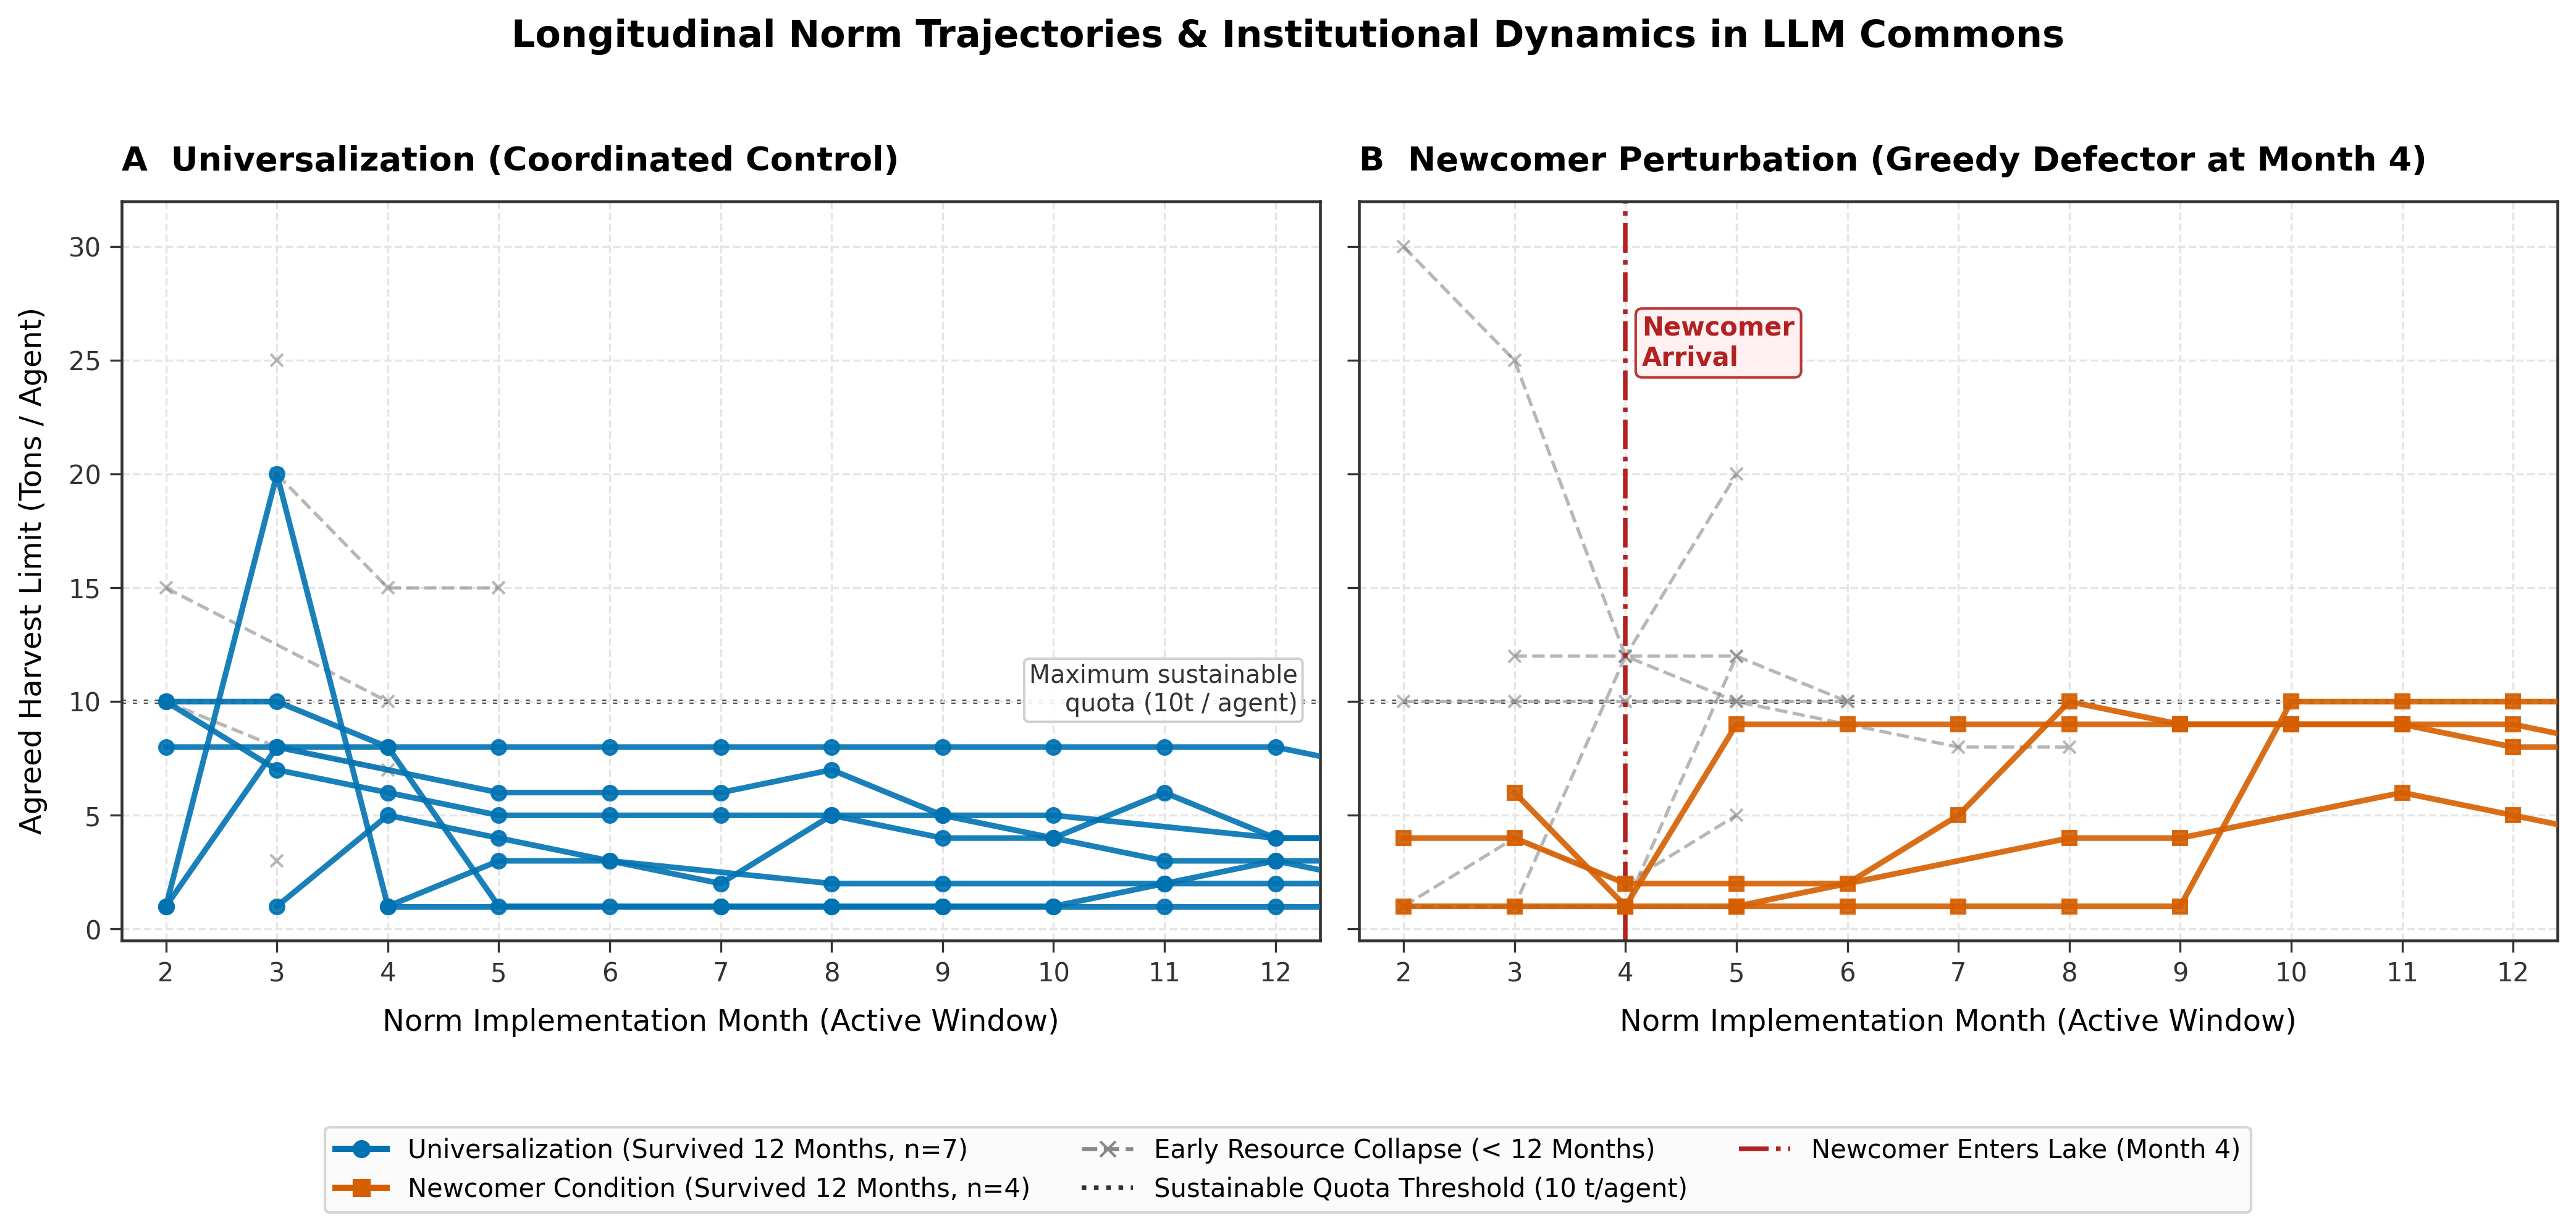
\includegraphics[width=0.95\textwidth]{norm_evolution/fig_norm_trajectories.png}
    \caption{\textbf{Trajetórias longitudinais dos limites acordados de colheita.} (A) Controles de universalização convergem monotonamente para limites conservadores (1--4t). (B) Após a entrada do newcomer no Mês 4 (linha tracejada vermelha), os sobreviventes exibem inflação de normas.}
    \label{fig:trajectories}
\end{figure}

Em total contraste, todos os 4 runs sobreviventes na condição com newcomer apresentaram slopes positivos ($+0,44$ a $+0,92$ t/mês, média de $+0,684$ t/mês; Fisher exato $p = 0,003$ vs controles; Mann-Whitney $p = 0,006$). Após a depleção violenta provocada pelo newcomer no Mês 4, as assembleias subsequentes fraturaram o consenso prudente, inflando os tetos acordados de volta para 8--10 toneladas/agente (Figura 1B). A Figura 2A destaca a nítida segregação em quadrantes entre o aperto conservador e a inflação desestabilizada.

\begin{figure}[htbp]
    \centering
    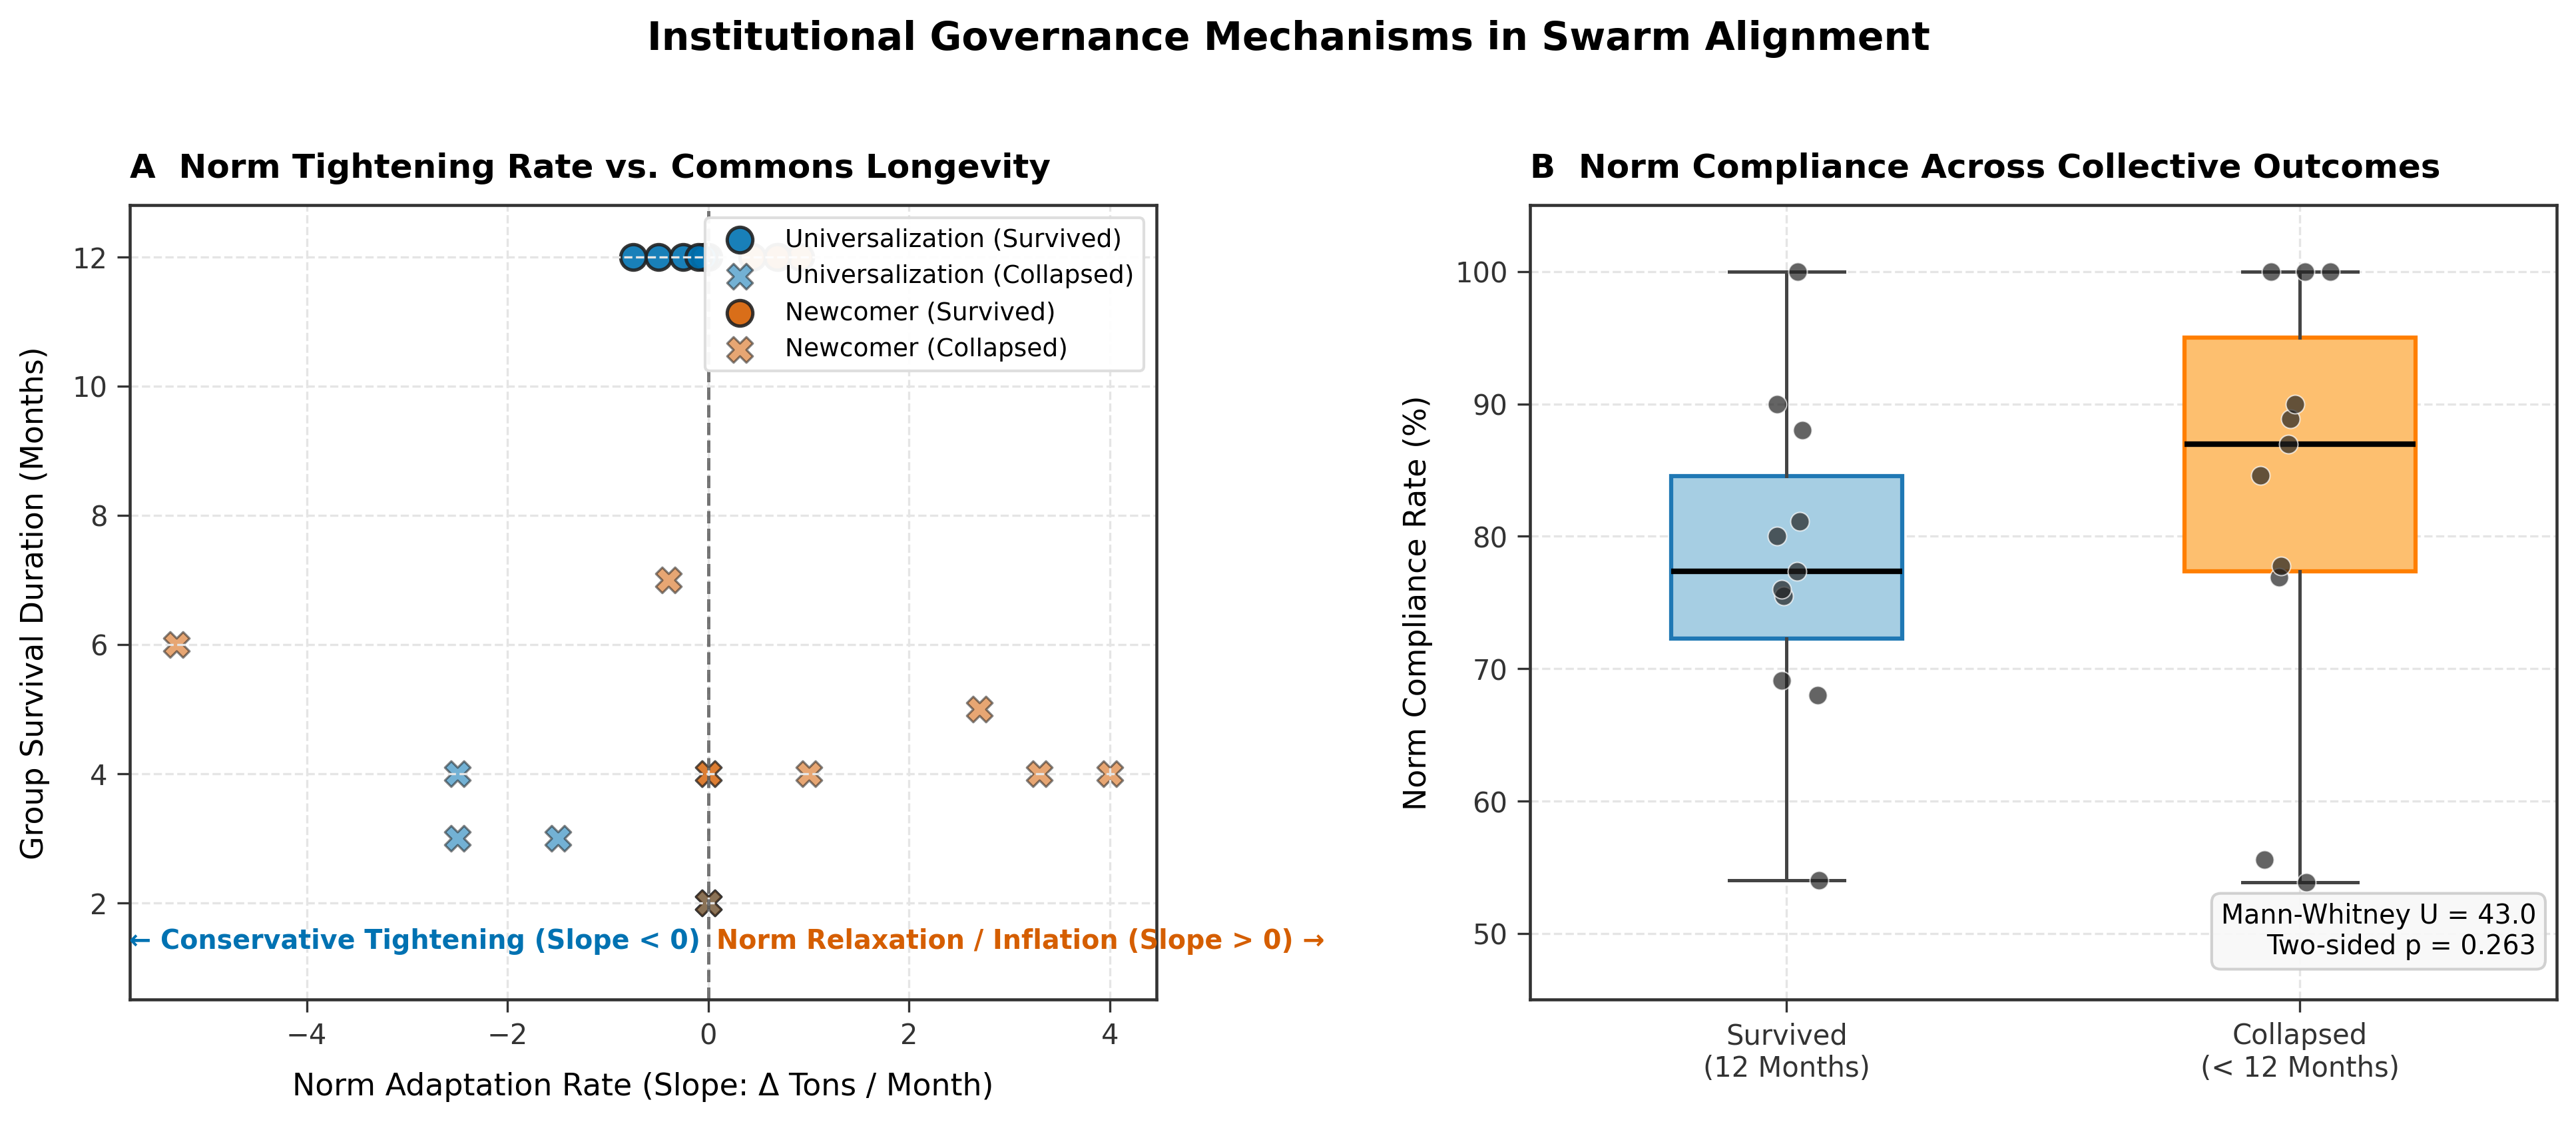
\includegraphics[width=0.92\textwidth]{norm_evolution/fig_tightening_and_compliance.png}
    \caption{\textbf{Mecanismos de governança institucional.} (A) Taxa de aperto normativo vs duração da sobrevida. (B) Elevadas taxas de conformidade entre grupos sobreviventes (78,1\%) e colapsados (83,1\%) ($p = 0,263$), comprovando que o colapso não decorre de trapaça interna.}
    \label{fig:compliance}
\end{figure}

Ao quantificar a conformidade (Figura 2B), os runs sobreviventes respeitaram os limites acordados em 78,1\% das oportunidades, enquanto os colapsados cumpriram a norma em 83,1\% dos casos (Mann-Whitney $U = 43,0, p = 0,263$). A inexistência de déficit de conformidade prova que os colapsos não ocorrem por quebra dissimulada de acordos entre membros; em contextos de ações simultâneas, o diálogo informal isolado carece de instrumentos sancionatórios capazes de deter a exaustão física do recurso.

\section{Discussão e Limitações}
\textbf{Implicações para o Alinhamento de Enxames:} Nossos resultados oferecem duas lições determinantes para a segurança de sistemas multiagente. Primeiro, LLMs dotados de comunicação formulam governança coletiva sofisticada: longe de seguir regras mecânicas rígidas, adaptam dinamicamente as restrições para erguer margens coletivas de segurança. Segundo, a vulnerabilidade de enxames alinhados é assimétrica: um agente malicioso deflagra o colapso sistêmico não por disseminar objetivos desregulados aos demais, mas ao explorar a latência de decisões simultâneas e quebrar a convergência institucional que sustentava o coletivo.

\subsection{Limitações Metodológicas}
\begin{enumerate}[leftmargin=*,itemsep=1pt]
    \item \textbf{Tamanho Amostral:} Com 13 runs por condição (7 vs 4 nos subgrupos com sobrevida), o poder estatístico é moderado, sustentando-se na expressiva magnitude de efeito acompanhada de valores de p limítrofes.
    \item \textbf{Assimetria Pré-Tratamento:} O GovSim inicializa a condição com newcomer com 4 agentes nos meses 1--3, criando viés de seleção mitigado estatisticamente pela análise de marco, porém inerente ao desenho experimental.
    \item \textbf{Deriva Linguística:} Em 7 runs (e.g., s4, s11), o modelo transitou parcialmente para o mandarim nos diálogos. Embora a extração quantitativa permaneça rigorosamente válida, citações qualitativas de diálogo devem priorizar simulações em inglês estrito (s1, s2, s3).
    \item \textbf{Arquitetura Única:} Os experimentos foram conduzidos estritamente no Qwen 2.5 7B. Embora comprove a viabilidade de modelos abertos leves na governança, a validação trans-arquitetura demanda estudos posteriores.
\end{enumerate}

\subsection{Trabalhos Futuros}
Constituem desdobramentos promissores: (1) O desenho de instrumentos sancionatórios descentralizados (votações, multas entre pares ou exclusão social) para implementar as sanções graduadas de Ostrom; (2) Protocolos sequenciais de apropriação para extinguir a vulnerabilidade de extração simultânea; e (3) Avaliação de enxames heterogêneos operando sob múltiplos pesos fundacionais distintos.

\section{Conclusão}
Em dilemas de recursos comuns, enxames cooperativos de LLMs desenvolvem governança institucional emergente, comprimindo adaptativamente as cotas de colheita para salvaguardar bens compartilhados. Todavia, esse alinhamento coletivo mostra-se frágil contra invasões predatórias: um único agente ganancioso induz severa mortalidade e desmantela a convergência normativa. Crucialmente, a falha manifesta-se sem contágio comportamental. Tais evidências atestam que a segurança em IA multiagente não pode repousar unicamente na benevolência comunicativa; o alinhamento robusto de enxames requer mecanismos institucionais verificáveis e imunes a atores não alinhados.

\section*{Código e Dados}
\textbf{Repositório de Código:} \texttt{[Placeholder de Link do GitHub: https://github.com/placeholder/swarm-alignment-govsim]} \\
\textbf{Dados / Artefatos:} Todos os registros de log, arquivos CSV de sobrevida, métricas de evolução de normas e figuras em alta resolução encontram-se arquivados no pacote de submissão (\texttt{norm\_evolution/}).

\section*{Contribuições dos Autores e Declaração de Trabalho Prévio}
\textbf{Contribuições dos Autores:} [O Autor 1 liderou o desenho experimental e a análise de evolução de normas. O Autor 2 executou as baterias de simulação em hardware local. Todos os autores participaram da interpretação, redação e revisão final do manuscrito.] \\
\textbf{Declaração de Trabalho Prévio (Triagem Apart Research):} Em estrita conformidade com as diretrizes do hackathon, demarcamos o trabalho prévio versus o do sprint:
\begin{itemize}[leftmargin=*,itemsep=1pt]
    \item \textit{Trabalho Prévio (Desenvolvido antes de 6 de novembro):} Scripts do ambiente GovSim local, patch de override ROCm no systemd, pipeline base de extração (\texttt{extract\_survival.py}, \texttt{km\_analysis.py}, \texttt{README\_original.md}).
    \item \textit{Trabalho do Fim de Semana do Sprint (7--8 de novembro):} Todas as 40 execuções completas de simulação, análise de contágio (\texttt{contagion\_analysis.py}), análise de marco do Mês 4 (\texttt{month4\_checks.py}) e o arcabouço completo de Evolução de Normas e Dinâmica Institucional (\texttt{analyze\_norm_evolution.py}, Figuras 1 e 2).
\end{itemize}

\section*{Limitações e Considerações Éticas / Uso Dual}
\textbf{Declaração Ética e de Uso Dual:} O presente estudo investiga a governança de bens comuns em simulação pesqueira computacional. Os achados não apresentam riscos biológicos, químicos, cibernéticos ou cinéticos diretos. Contudo, emergem implicações de uso dual relativas a operações descentralizadas: demonstrar que espaços de ação simultânea são vulneráveis à extração pontual irreversível pode subsidiar estratégias oportunistas contra protocolos descentralizados autônomos (como pools de liquidez DeFi ou clusters compartilhados de computação). Ao documentar com rigor essa vulnerabilidade, enfatizamos a urgência de mecanismos criptográficos de verificação, compromissos sequenciais e sanções estruturais na infraestrutura autônoma multiagente.

\section*{Referências}
\begin{enumerate}[leftmargin=*,itemsep=2pt]
    \small
    \item Dafoe, A., Bachrach, Y., Hadfield, G., Horvitz, E., Larson, K., \& Graepel, T. (2020). Cooperative AI: machines must learn to find common ground. \textit{Nature}, 581(7806), 32--34.
    \item Hardin, G. (1968). The Tragedy of the Commons. \textit{Science}, 162(3859), 1243--1248.
    \item Leibo, J. Z., Zambaldi, V., Lanctot, M., Marecki, J., \& Graepel, T. (2017). Multi-agent reinforcement learning in sequential social dilemmas. In \textit{Proceedings of the 16th Conference on Autonomous Agents and MultiAgent Systems (AAMAS)}, 464--473.
    \item Mekhalfi, M. L., et al. (2024). Exploring Social Dilemmas in Multi-Agent Large Language Models. \textit{arXiv preprint arXiv:2403.00123}.
    \item Ostrom, E. (1990). \textit{Governing the Commons: The Evolution of Institutions for Collective Action}. Cambridge University Press.
    \item Park, J. S., O'Brien, J. C., Cai, C. J., Morris, M. R., Liang, P., \& Bernstein, M. S. (2023). Generative agents: Interactive simulacra of human behavior. In \textit{Proceedings of the 36th Annual ACM Symposium on User Interface Software and Technology (UIST)}, 1--22.
    \item Piatti, G., Frank, T. P., Zhang, J., \& Puzicha, J. (2024). GovSim: Can Large Language Models Govern the Commons? \textit{arXiv preprint arXiv:2402.18567}.
\end{enumerate}

\section*{Apêndice: Declaração de Uso de LLMs}
\textbf{Declaração de Uso de Ferramentas de IA:} Assistentes de linguagem (Claude e Gemini) foram utilizados para brainstorm de formulações estatísticas, estruturação de código dos scripts, depuração de logs e apoio na redação acadêmica. Todas as simulações, métricas numéricas, testes estatísticos e figuras visuais foram executados, conferidos e validados de maneira independente pelos autores com base nos logs brutos.

\end{document}
